\chapter{弧度制}
\label{ch:Circular Measure}
现在你们要学习高级一点的角度表示方法了。就像小时候采用$1,2,3$这样的数字系统,到了高中之后采用$x,y,z$这样的代数系统。描述角度新的方法就是\gls{radians}
\begin{figure}[H]
\centering
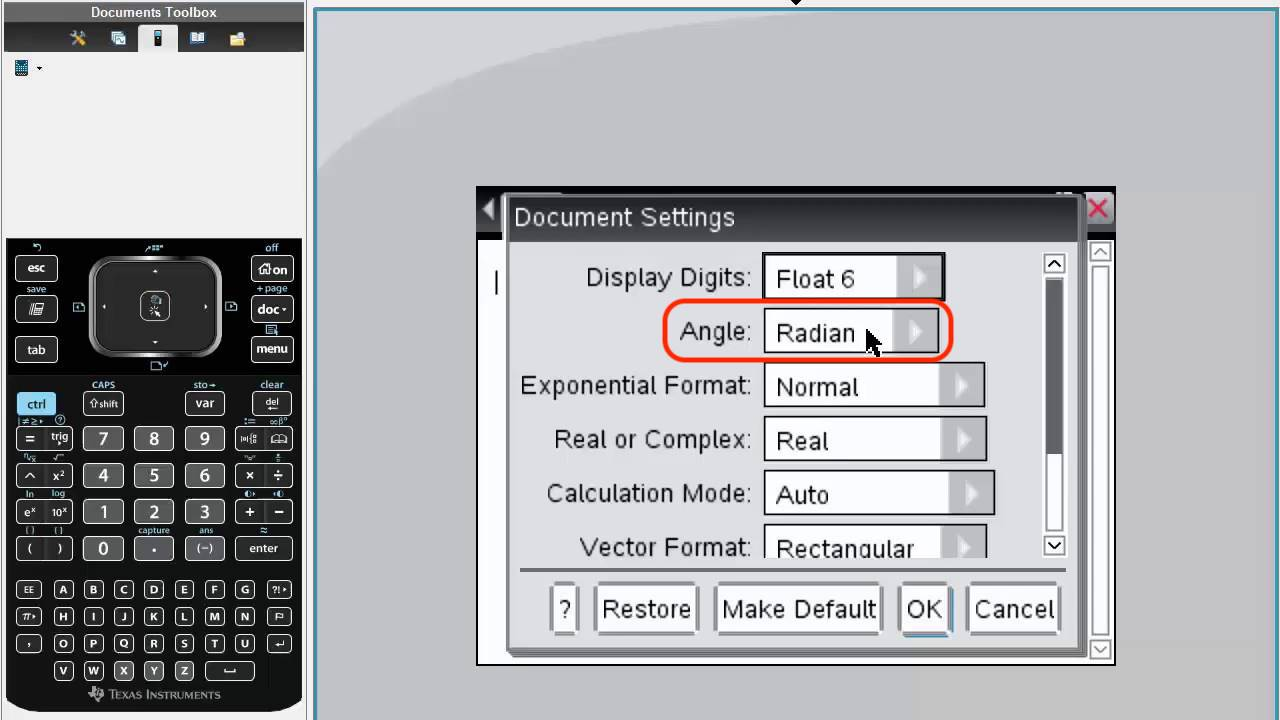
\includegraphics[width=0.8\textwidth]{calc-radian}
\caption{TI-nspire当中角度度量的选择}
\end{figure}


\section*{学习目标}
\begin{todolist}
 \item 理解角度制和弧度制作为衡量一个角大小的测度系统
 \item 记忆和运用弧度制的定义和相关公式
 \item 对一个角的弧度制和角度制结果实现互相转化
 \item 利用弧度制求算扇形的弧长以及面积,解决其他相关问题
\end{todolist}
\clearpage


\section{弧度}
\label{sec:Radian}
我们之前定义$1$\si{\degree}的角是通过:将一个\gls{pangle}做180等分,每一份的角就是$1$\si{\degree}。因此在这种角度制的体系下,角的大小是携带有``\si{\degree}''这样的单位的。

而现在新的体系下,我们将角放入到扇形当中,用扇形的弧长和半径之比作为该角的大小。
\begin{figure}[H]
\centering
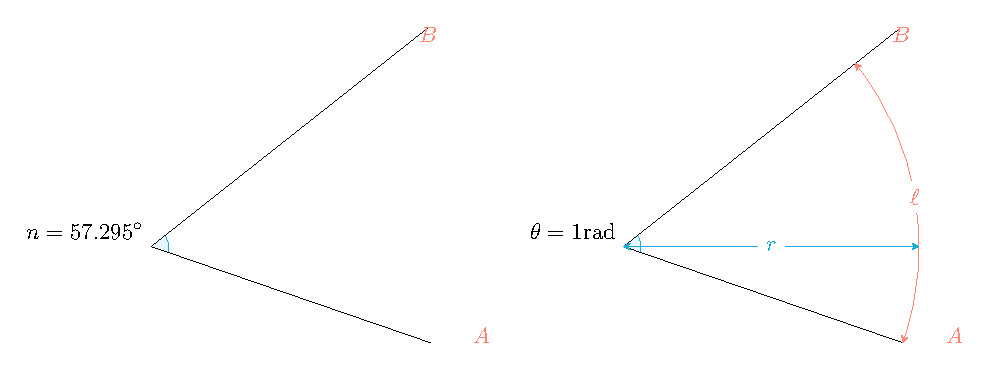
\includegraphics[width=0.8\textwidth]{DegRad} 
\caption{度数制系统和弧度制系统}
\end{figure}

因此我们定义一个角的弧度制的定义是:
\[
	\theta=\frac{\ell}{r}
\]

\subsection*{弧度制与度数制的转换关系}
\label{subsec: Convertion between Radians and Degrees}
根据定义,一个$180$\si{\degree}的角,安置在扇形中,其弧长为$\frac{1}{2}\cdot 2\pi r$。因此平角的弧度为$\frac{\frac{1}{2}\cdot 2\pi r}{r}=\pi$。这就是我们对弧度制和度数制的基本转换关系:
\[
	180\si{\degree} = \pi \text{ rad} \approx 3.141592 \text{ rad}
\]
因此任意任意角度$n$\si{\degree}都可以转化为对应的弧度$\theta$。转化公式如下:

\begin{align*}
	\theta &=\frac{\frac{n \si{\degree}}{360\si{\degree}}\cdot 2\pi r}{r} \\
			&=\frac{n \si{\degree}}{360\si{\degree}}\cdot 2\pi\\
			&=\frac{n \si{\degree}}{180\si{\degree}}\cdot \pi\\
			&=n\si{\degree} \cdot \frac{\pi}{180\si{\degree}}
\end{align*}

那么,如果将弧度制的角转变为度数制的角的话,则是一个相反的逆过程:
\[
	n\si{\degree} =\theta \cdot \frac{180\si{\degree}}{\pi}
\]

由此,稍微记牢一下常见的特殊角对应的角度制和弧度制数值。
\begin{table}[H]
\centering
\begin{tblr}{
	colspec={|l|[2pt,dotted]c|c|c|c|c|c|c|c|c|c|},
	hspan=0.7\textwidth
	}
\hline
Deg & 0\si{\degree} & 30\si{\degree} & 45\si{\degree} & 60\si{\degree} & 90\si{\degree} & 120\si{\degree} & 150\si{\degree} & 180\si{\degree} & 270\si{\degree} & 360\si{\degree} \\ 
\hline 
Rad & 0 & $\quad$ & $\quad$ & $\quad$ & $\quad$ &$\quad$ & $\quad$& $\pi$&$\quad$  & $2\pi$\\ 
\hline
\end{tblr}
\end{table}


\begin{TaskBox}
完成表格当中空余的部分
\tcblower 
思考这些表格中的$\pi$是不是弧度制的单位?或者说弧度制有没有单位?
\end{TaskBox}
\clearpage


\section{扇形性质}
\label{sec:Property of Sector}
对于一个扇形,当已知该扇形的圆心角(以弧度制记)和半径之后,其弧长的求算公式为:
\[
	\ell =r\cdot \theta
\]
而对于其面积,求算公式为:
\begin{align*}
	A &= \frac{\theta}{2\pi} \cdot \pi r^2 \\
		&=\frac{1}{2} r^2\theta\\
		&=\frac{1}{2}r \cdot \ell
\end{align*}
而如果是扇形的弦长的话,其长度的求算公式则为:
\[
	\text{chord length} =2r\cdot \sin \left(\frac{\theta}{2}\right)
\]

如下图所示,所有的求算结果都标记出来的
\begin{figure}[H]
\centering
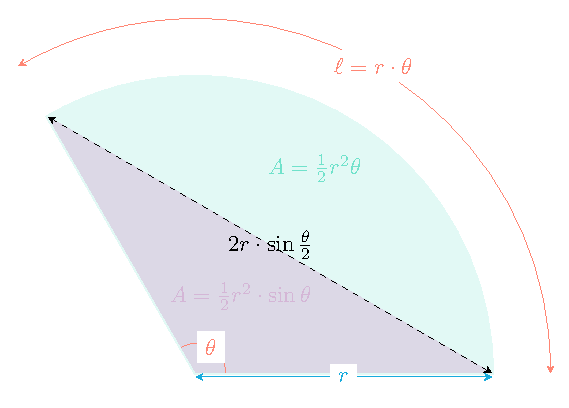
\includegraphics[width=0.8\textwidth]{sector}
\caption{扇形中的各种求算}
\end{figure}


\clearpage

